\section{Trigonometric Functions and Triangles}\label{sec:trig_triangles}

In this section, we will further discuss trigonometric functions. We will examine the relationship between trigonometric functions and right triangles, and examine some more properties of trigonometric functions.

\vskip \baselineskip
\noindent\textbf{\large Right Triangles}\\

In the last section, we focused on the relationships between the trigonometric functions and the unit circle. Now, we will examine the relationship of these functions and the unit circle with right triangles. In Figure \ref{fig:triangle_in_unitcircle}, we start by drawing a unit circle with an angle $\theta$ and marking the corresponding coordinates on the circle. If we drop down from these coordinates to the x axis, we can form a right triangle. 

\begin{figure}[H]
	\centering
	\vskip 0in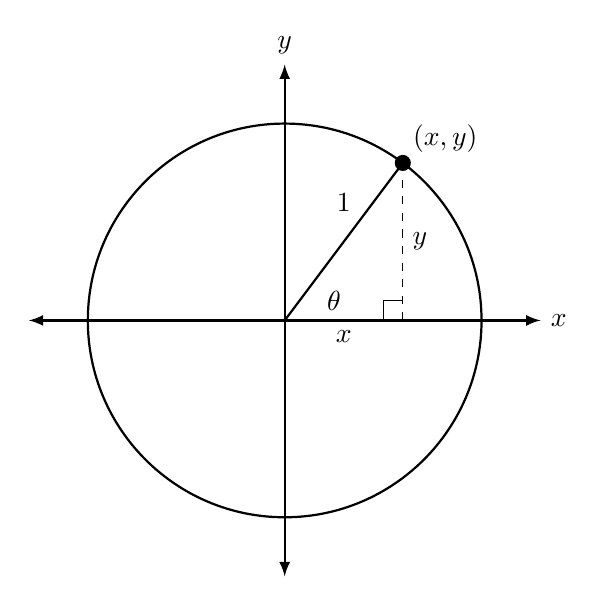
\begin{tikzpicture}[>=latex,scale=2.5,thick]
\draw [<->](-1.3,0)--(1.3,0) node [right] {$x$};
\draw [<->] (0,-1.3) -- (0,1.3) node [above] {$y$};
\draw (0,0) circle (1);
\draw [fill= black] (.6,.8) circle (1pt);
\draw (0,0) -- (.6,.8) node [above right] {$(x,y)$};
\draw [dashed,thin] (.6,.8) -- (.6,0) node [pos=.5,right] {$y$};
\draw (.3,0) node [below] {$x$};
\draw (.3,.6) node {$1$};
\draw (.25,.1) node {$\theta$};
		\draw [thin] (.5,0) -- (.5,.1) -- (.6,.1);
\end{tikzpicture}
\caption{Right triangle inside of the unit circle}\label{fig:triangle_in_unitcircle}
\end{figure}

This triangle has a hypotenuse of 1 because the hypotenuse is the same length as the radius of the unit circle, and side lengths of $x=\cos{(\theta)}$ and $y=\sin{(\theta)}$. If we apply the Pythagorean Theorem to this triangle, we discover an interesting identity:

\begin{equation}
	\begin{split}
		a^2 + b^2 & = c^2 \\
		(x)^2 + (y)^2 & = (1)^2 \\
		(\cos{(\theta)})^2 + (\sin{(\theta)})^2 &= 1^2 \\
		\cos^2{(\theta)} + \sin^2{(\theta)} & = 1
	\end{split}
\end{equation}

There is nothing special about the choice of $\theta$ shown in Figure \ref{fig:triangle_in_unitcircle}; this identity is true for all inputs. Notice that the input for cosine and the input for sine are the same; if the inputs are different, we cannot guarantee that the sum will be equal to 1.

This right triangle also gives us a different way of evaluating trigonometric functions, in general. With the unit circle, we saw that $\cos{(\theta)}$ is the x coordinate and $\sin{(\theta)}$ is the y coordinate, and our right triangle has a hypotenuse of 1. If we scale the triangle, the side lengths will also scale, but the size of the angles will remain the same, so the values of $\cos{(\theta)}$ and $\sin{(\theta)}$ should also remain the same. In order for this to be true, we can't just say that cosine is the length of the adjacent side and sine is the length of the opposite; instead, we will need to divide both by the length of the hypotenuse to adjust for the scaling (see Figure \ref{fig:right_triangle} for a visual explanation of the opposite and adjacent sides). This gives us the following identities:

\begin{figure}[H]
	\centering
	\vskip 0in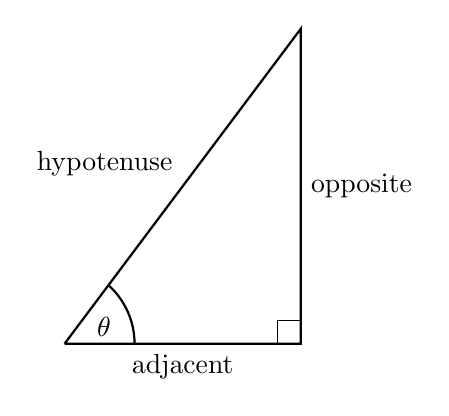
\begin{tikzpicture}[thick]
		\draw (0,0) -- (3,0) -- (3,4) -- (0,0);
		\draw (.5,.22) node {$\theta$};
		\draw (1.5,0) node [below] {adjacent};
		\draw (3,2) node [right] {opposite};
		\draw (1.5,2) node [above left] {hypotenuse};
		\draw [-] (.88888888,0) arc (0:48:1);
		\draw [thin] (2.7,0) -- (2.7,0.3) -- (3,0.3);
\end{tikzpicture}
	\caption{Using a right triangle to evaluate trigonometric functions}\label{fig:right_triangle}
\end{figure}


\noindent
\begin{minipage}[t]{.5\textwidth}
		\begin{enumerate}
		\item	$\sin{(\theta)} = \frac{\text{opposite}}{\text{hypotenuse}}$	
		\item	$\cos{(\theta)} = \frac{\text{adjacent}}{\text{hypotenuse}}$
		\item	$\tan{(\theta)} = \frac{\text{opposite}}{\text{adjacent}}$		
		\end{enumerate}
		\end{minipage}
		\begin{minipage}[t]{.5\textwidth}
		\begin{enumerate}\addtocounter{enumi}{3}
		\item	$\csc{(\theta)} = \frac{\text{hypotenuse}}{\text{opposite}}$
		\item	$\sec{(\theta)} = \frac{\text{hypotenuse}}{\text{adjacent}}$			
		\item	$\cot{(\theta)} = \frac{\text{adjacent}}{\text{opposite}}$
		\end{enumerate}	
		\end{minipage}

Many people summarize the first three of these with SOH-CAH-TOA to help remember the identities. SOH-CAH-TOA stands for Sine is Opposite over Hypotenuse; Cosine is Adjacent over Hypotenuse, and Tangent is Opposite over Adjacent. The remaining three identities can then be formed from the definitions of cosecant, secant, and cotangent. Let's take a look at how we can use right triangles to help us evaluate our trigonometric functions.

\vskip \baselineskip

\example{ex_trig_right_triangle}{Using a Right Triangle}{Suppose that $\cos{(\theta)} = \frac{12}{13}$. Determine all possible values of $\sin{(\theta)}$.}{To help find the possible values of $\sin{(\theta)}$, we will draw a right triangle and label it using the values we already know. We know that $\cos{(\theta)} = \frac{12}{13}$, so we can use 12 as the length of the adjacent side and 13 as the length of the hypotenuse:
	\vskip 0in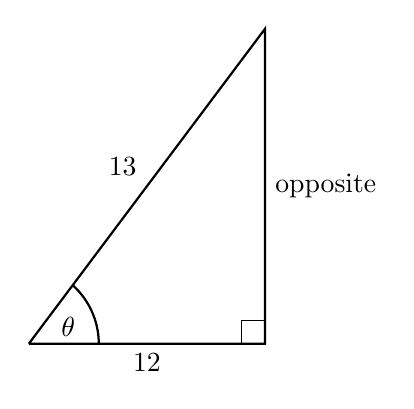
\begin{tikzpicture}[thick]
		\draw (0,0) -- (3,0) -- (3,4) -- (0,0);
		\draw (.5,.22) node {$\theta$};
		\draw (1.5,0) node [below] {12};
		\draw (3,2) node [right] {opposite};
		\draw (1.5,2) node [above left] {13};
		\draw [-] (.88888888,0) arc (0:48:1);
		\draw [thin] (2.7,0) -- (2.7,0.3) -- (3,0.3);
\end{tikzpicture}

Now, we can use the Pythagorean Theorem to find the missing side length:

\begin{equation*}
	\begin{split}
		a^2 + b^2 &= c^2 \\
		(12)^2 + b^2 & = 13^2 \\
		144 + b^2 & = 169 \\
		b^2 & = 25 \\
		b & = \pm5
	\end{split}
\end{equation*}

Now, we can update our drawing:

	\vskip 0in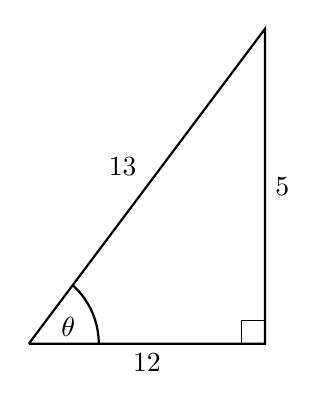
\begin{tikzpicture}[thick]
		\draw (0,0) -- (3,0) -- (3,4) -- (0,0);
		\draw (.5,.22) node {$\theta$};
		\draw (1.5,0) node [below] {12};
		\draw (3,2) node [right] {5};
		\draw (1.5,2) node [above left] {13};
		\draw [-] (.88888888,0) arc (0:48:1);
		\draw [thin] (2.7,0) -- (2.7,0.3) -- (3,0.3);
\end{tikzpicture}

In our drawing, we labeled all of the sides with positive values because when we measure the side of a triangle we will get a positive length. From this triangle, we get $\sin{(\theta)} = \frac{\text{opposite}}{\text{hypotenuse}} = \frac{5}{13}$. However, this is not the only possible value of $\sin{(\theta)}$. We do not know the true value of $\theta$ and in our drawing assumed that it is between 0 and $\frac{\pi}{2}$. In reality, it could also be between $\frac{3\pi}{2}$ and $2\pi$. This would mean that $\sin{(\theta)}$ could also have a negative value. 
	\begin{center}
		\begin{tabular}{| c |} \hline
			\\[-4pt]
			The possible values of $\sin{(\theta)}$ are $\dfrac{5}{13}$ and $-\dfrac{5}{13}$ \\[-4pt]
			\\\hline
		\end{tabular}
	\end{center}}\\

\vskip \baselineskip
\noindent\textbf{\large Inverse Trigonometric Functions}\\

Often, we will have information about the side lengths of the triangle, but will want to know the value of the angle. This is where we will need the inverse trigonometric functions. Each trigonometric function has an inverse, but the inverses of sine, cosine, and tangent are the most commonly used. The notation for the functions is a bit tricky. We've seen that we can write $(\sin{(\theta)})^2$ as $\sin^2{(\theta)}$, however, the notation $\sin^{-1}{(\theta)}$ is often used to represent the inverse sine function rather than the function $\frac{1}{\sin{(\theta)}}$. In this book, we will instead use the notation $\arcsin{(x)}$ to represent the inverse sine function. This eliminates confusion over notation, but you should be aware that not all references do this. Similarly, we use $\arccos{(x)}$ for the inverse cosine function and $\arctan{(x)}$ for the inverse tangent function. These can be referred to as arcsine, arccosine, and arctangent in writing.

Notice that for each of these inverse trigonometric functions, we used $x$ as our input rather than $\theta$. This is because we are no longer inputting an angle, but rather a ratio of lengths. For these functions, our output will be an angle. Remember, when we say that two functions are inverses, we mean that there is a relationship like the following: $\arccos{(\cos{(\theta)})}=\theta$ and $\cos{(\arccos{(x)})} = x$. Another way of expressing this relationship is to say that if $\cos{(\theta)} =x$, then $\arccos{(x)} = \theta$. However, this is not exactly true here. When we look at trigonometric functions, we know that there are lots of angles that all result in the same value for sine, lots of angles that result in the same value for cosine, and lots of angles that result in the same value for tangent. Because we only want one output for each input, the inverse trigonometric functions use restricted outputs. Arccosine is restricted to output values between $0$ and $\pi$, meaning that its range is $[0,\pi]$. This works because every possible output of cosine shows up once for angles from 0 to $\pi$. Arcsine and arctangent are restricted to output values between $-\frac{\pi}{2}$ and $\frac{\pi}{2}$, meaning that they each have a range of $[-\frac{\pi}{2}, \frac{\pi}{2}]$. For both tangent and sine, every possible output value appears once for angles between $-\frac{\pi}{2}$ and $\frac{\pi}{2}$. By restricting the ranges, we make sure these functions are well-defined, meaning they only produce one output for each input.

In practice, we can still use the unit circle to help evaluate inverse trigonometric functions. For example, if we want to evaluate $\arcsin{(\frac{1}{2})}$, we will want to look at the unit circle to see where $\sin{(\theta)}=\frac{1}{2}$. We get two angles: $\frac{\pi}{6}$ and $\frac{5\pi}{6}$. Since the range of arcsine is restricted to $[-\frac{\pi}{2},\frac{\pi}{2}]$, we say that $\arcsin{(\frac{1}{2})} = \frac{\pi}{6}$. Similarly, we would say that $\arccos{(\frac{1}{2})} = \frac{\pi}{3}$, and $\arctan{(1)} =\frac{\pi}{4}$.


\printexercises{exercises/trig_triangles_exercises}


%\clearpage
